\chapter[What may I hope?]{What may I hope? \newline {\fontsize{18}{32}\selectfont General discussion and future perspectives}}
\chaptermark{What may I hope?}
\label{chap:discussion}

{ \Large \leftwatermark{
		\put(-67,-66.5){ 1 }
		\put(-67,-91.5){ 2 }
		\put(-67,-116.5){ 3 }
		\put(-67,-141.5){ 4 }
		\put(-67,-166.5){ 5 }
		\put(-67,-191.5){ 6 }
		\put(-67,-216.5){ 7 }
		\put(-67,-241.5){ 8 }
		\put(-67,-266.5){ 9 }
		\put(-67,-291.5){ 10 }
		\put(-76.5,-325){
\includegraphics[scale=0.8]{img/thumbindex.eps}} \put(-67,-316.5){ {\color{white} 11 }}
		
	} \rightwatermark{
		\put(350.5,-66.5){ 1 }
		\put(350.5,-91.5){ 2 }
		\put(350.5,-116.5){ 3 }
		\put(350.5,-141.5){ 4 }
		\put(350.5,-166.5){ 5 }
		\put(350.5,-191.5){ 6 }
		\put(350.5,-216.5){ 7 }
		\put(350.5,-241.5){ 8 }
		\put(350.5,-266.5){ 9 }
		\put(350.5,-291.5){ 10 }
		\put(346.5,-325){
\includegraphics[scale=0.8]{img/thumbindex.eps}} \put(350.5,-316.5){ {\color{white} 11 }}
}}


\newpage


In this thesis I have improved applications of next-generation sequencing (NGS) DNA analysis for the detection of different variant types. 
However, the detection of variants is only a part, albeit an important part, of the process of DNA diagnostics. 
After detection, clinical interpretation of the variants is the next step before reporting test results to the clinic. 
There are many ways to improve the interpretation process, and this is also the subject of ongoing studies within our own department. 
For the purpose of this discussion, I will focus primarily on the potential gains to be made in improving variant detection and using alternative DNA sequencing approaches. 
I will first discuss what each part of this thesis contributed to the field of genetic variant detection (11.1-11.3).
Then I will examine the relation between laboratory procedures and data analysis (11.4). 
Finally, I will discuss the benefits of available sequencing techniques for detection of different variant types (11.5-11.6) and provide ideas on possible future directions (11.7).

\section{Germline variant testing} \label{Germline}
In \textbf{chapter 2} of this thesis we describe our introduction of NGS, or massively parallel sequencing, as a replacement for Sanger sequencing in clinical diagnostics. 
Before this, Sanger sequencing was the standard in DNA sequencing for Single Nucleotide Variant (SNV) and indel detection. 
Making use of the Miseq sequencer from Illumina, we designed a panel of genes (initially 48) associated with cardiomyopathies. 
Our targeted NGS (tNGS) approach was implemented in genome diagnostics in the first half of 2013, which made us a frontrunner in the introduction of NGS as first-line test in routine genetic diagnostics. Because (all) relevant genes could be sequenced in parallel in a single test, lead times were substantially decreased and more patients received a diagnosis. 
Following the cardiomyopathy gene panel approach, we designed other panels targeting genes related to other hereditary conditions, such as familial cancer, genetic skin diseases and epilepsy.

Because, initially, only SNVs and small indels could be detected using our tNGS approach, multiplex-ligation dependent probe amplification (MLPA) was used to complement our analysis with detection of copy number variants (CNVs). 
Unfortunately, like Sanger sequencing, MLPA can only analyze a limited set of targets in a single experiment. 
Although tools were available to detect CNVs from NGS data, such as CoNIFER \cite{Krumm_2012}, XHMM \cite{Fromer_2012} and ExomeDepth \cite{Plagnol_2012}, these tools were based on analysis of read depth and had been created for exome data with a focus on research rather than diagnostics. 
These tools generally focus on detection of multi-exon CNVs with optimal sensitivity and specificity. 
In contrast, in targeted capturing, indel callers can only detect variants smaller than an exon. 
Because the entire exon is affected, no breakpoint information is available for those CNVs, which makes these variants impossible to detect by indel callers such as the GATK Haplotype caller \cite{van_der_Auwera_2013}.
Single-exon CNVs are thus too small for CNV detection tools, but too large for indel callers to detect.
In diagnostics, however, there is also a need to detect variants at a single-exon level with high sensitivity and specificity and to see for which exons a reliable prediction can be made, particularly because known founder mutations consisting of a single-exon CNV are present in some cases \cite{Bayley_2009,Petrij_Bosch_1997}. 
In other words, a \underline{negative result} needs to be distinguished from \underline{no result}. 
For this reason, in \textbf{chapter 3}, we introduced CoNVaDING, a tool optimized for the detection of single-exon germline CNVs in high-coverage tNGS data. 
CoNVaDING adds to the existing CNV detection toolbox by providing exon-specific quality metrics. 
Furthermore, the algorithms on which CoNVaDING is based take a different perspective than the other tools on the noise that affects read depth between samples and sequence runs, and therefore uses different strategies for
reduction of variation in exon read-depth between samples. 
Because of these different noise reduction strategies, false positive and false negative results will often differ between tools. 
We have shown in \textbf{chapters 3 and 4} that combining CoNVaDING and XHMM in a joint prediction strategy further increases the sensitivity and specificity of CNV analysis. 
With the addition of CNV detection in tNGS analysis, we have taken a further step towards an all-in-one test for genetic variant detection.
In \textbf{chapter 4} we show that, when combining all indications in hereditary cancer diagnostics, CNV detection adds 0.6\% diagnostic yield to the 9.5\% of pathogenic and likely pathogenic variants detected at single nucleotide level.

Currently, it is being heavily debated in the literature if, and which, secondary findings should be returned to clinical genetics patients \cite{Hart_2018,Kalia_2016,Pujol_2018,Mackley_2016,Shkedi_Rafid_2014,Wouters_2018,van_El_2013}. 
In \textbf{chapter 4}, I take one step back and show which secondary findings are present in the genes tested in our hereditary cancer gene panel for both Dutch patients referred for hereditary cancer and members of
the general Dutch population. 
Here we found that approximately 3\% of people carry a (likely) pathogenic variant in one of these genes. 
Following the ACMG \cite{Green_2013,Kalia_2016} or SFMPP \cite{Pujol_2018} guidelines, 0.7\% and 1.4\%, respectively, of people tested with the hereditary cancer gene panel carry a (likely) pathogenic variant for which there is enough evidence for clinical utility to indicate that they should be reported back to the patients. 
With our research we provide context for the debate on reporting secondary variants and screening for those findings.
Whereas our research focused only on genes related to hereditary cancer, our findings add to the general discussion on the desirability of screening for pathogenic variants.


\sectionmark{Somatic chromosomal translocations} % extra to get the top mark okay..
\section{Detection of somatic chromosomal \newline translocations} \label{Somatic}
\sectionmark{Somatic chromosomal translocations}
Using standard short-read sequencing, it is usually impossible to detect copy-neutral structural variations. 
In part 2 of the thesis (\textbf{chapter 5}), we adapted the NGS short-read sequencing sample preparation protocol to detect translocations, making use of Targeted Locus Amplification (TLA) technology \cite{de_Vree_2014}. 
TLA connects and amplifies DNA regions that are spatially close to each other through cross-linking, digestion and ligation. 
This is ideal for translocation detection because parts of chromosomes are spatially relocated in a translocation. 
If a gene on one of the chromosomes involved is targeted using TLA, DNA of the translocation partner chromosome is amplified too. 
Therefore, even though the reads themselves are only a few hundred base pairs long, the sequences of the translocation partner are present. 
After alignment, those reads show up as a peak in a sequence coverage plot of the genome. 
In the standard procedure, a single gene is targeted in a single TLA experiment. 
We expanded the number of targeted loci to 18 genes to create a panel for translocation detection in acute leukemia. 
This means that the reads of cross-linked DNA of all 18 genes and nearby regions are present within the data of a single experiment. 
If an extra peak is present due to a translocation, the peak could be the translocation partner of any of the 18 genes in the panel. 
We therefore created an analysis workflow that includes novel algorithms to cope with the mixed data. In this analysis, aligned reads are split into subsets based on the targeted genes, followed by a series of steps to filter out noise, then the detection of peaks. 
The noise reduction is critical to achieve a high specificity and sensitivity. Unfortunately, we could not achieve optimal sensitivity using noise canceling because, when a translocation is present in only a low percentage of cells, the peak size will be smaller than noise peaks. 
A further limitation of TLA in the detection of SVs is that it is hard to control cross-linking strength and get the optimal experiment. 
If cross-linking is too weak, only DNA within a limited distance of the targeted locations is captured, which lowers sensitivity because fewer reads of the translocation partner chromosome are present. 
If cross-linking is too strong, a high level of noise will be present because large chromosomal areas around targeted genes are amplified. 
This lowers specificity and thereby sensitivity. 
In principle our panel can also be used for the detection of inversions, but at low specificity because of variable cross-linking efficiencies. 
Currently, in our opinion, the TLA multiplex-panel is not suitable for introduction into diagnostics. 
High-quality input material and standardization of laboratory procedures may create more stable results and allow for further optimization of protocols. 
However, Cergentis was recently awarded a European Research Council Horizon 2020 grant to optimize and validate the TLA technology for the analysis of FFPE tumor biopsies. 
This optimization may also benefit the multiplex-panel data quality \cite{Cergentis_2018}.

\section{Prenatal detection of trisomies} \label{Prenatal}
In part 3 of this thesis I focused on prenatal detection of trisomies, more specifically on non-invasive prenatal testing (NIPT) using low-coverage WGS. 
In \textbf{chapter 6}, we improved NIPT data-analysis by introducing three novel algorithms: the chi-squared-based variation reduction ($\chi$\textsuperscript{2}VR), the regressionbased Z-score (RBZ) and the Match QC score. 
By determining if there is more variation than can be expected by chance, the regions that create variability between samples can be accurately determined and corrected for using $\chi$2VR.
In addition, we have turned some of the bias present in NIPT data to our advantage by creating the RBZ, the first trisomy prediction algorithm that makes use of inverse correlation between chromosomal fractions (e.g if fewer reads are present on chromosome 13, more reads are present on chromosome 19).
This means that, even without any noise correction, the RBZ can already make an accurate prediction. 
In addition, the Match QC score indicates whether the control group being used is not suitable for the analysis of a specific sample. 
In combination, these algorithms allow for optimal comparison of a sample with control samples. 
In \textbf{chapter 7}, we make these algorithms available as the \textsl{NIPTeR} R package, together with other published algorithms for low-coverage WGS NIPT analysis. 
In \textbf{chapter 8}, we transform the NIPT result into a personalized posterior risk in order to aid a clinical interpretation an NIPT analysis outcome.

In the past few years NIPT has developed from being a test that was not allowed in the Netherlands into becoming the standard first-line test in the screening for prenatal trisomies. 
When I first started my work on NIPT (before I started my PhD) and visited Leiden in 2011 to learn the procedures and interpretation of results, it was still three years prior to the start of the TRIDENT-1
study that allowed NIPT in the Netherlands under strict criteria for women with a high risk of carrying a child with a trisomy \cite{MeeroverNIPT_2018}. 
During this period, Dutch women not eligible for testing went to Belgium to undergo NIPT \cite{Visser_2014} because it allowed for prenatal trisomy detection without the risk of inducing miscarriage. 
This situation changed when the TRIDENT-2 study started in 2017 and NIPT became available to all pregnant women in the Netherlands. 
By the following year, 42\% of pregnant women in the Netherlands had opted for an NIPT \cite{niptconsortium_2018}. 
Until NIPT was discontinued in the UMCG genome diagnostics laboratory because the analysis was centralized in the Netherlands, our NIPT data analysis was based on \textsl{NIPTeR} and \textsl{NIPTRIC}.

\sectionmark{Balancing lab procedures and data analysis} % extra to get the top mark okay..
\section[Balancing laboratory procedures and data analysis]{The intricate balance between laboratory \newline procedures and data analysis}\label{Balance}
\sectionmark{Balancing lab procedures and data analysis}
The methods and algorithms introduced in this thesis all focus on different topics and are based on different types of input data. 
Detection of each type of variant asks for a different approach, both in sample preparation and in the analysis and interpretation, to overcome the four types of noise 
discussed in chapter 9: biological, laboratory-induced, sequencing and data analysis. 
The analysis algorithms are closely tied to the exact data produced in the laboratory. 
Moreover, they should be seen as an extension of the laboratory procedure, although different analysis algorithms may detect different types of variants in the same data by taking a different perspective (e.g. order of
nucleotides in aligned reads to detect SNVs or read-depth to detect CNVs). 

\begin{figure}
	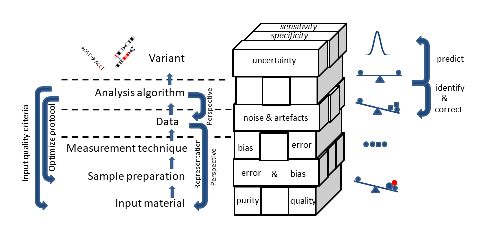
\includegraphics[width=1.0\linewidth]{img/Chapter11_fig1}
	\caption[Workflow of laboratory procedures and variant detection]{\textbf{Abstracted workflow of laboratory procedures and variant detection.} The DNA sequence of interest is represented by the blue circles. The input material can be impure (e.g. mixed tumor and normal cells) as represented by the red circle, or of low quality (e.g. fragmented DNA or DNA in which base changes have occurred through transversion (i.e. C $\leftrightarrow$ A or G $\leftrightarrow$ T change)) as represented by the larger blue circle. DNA from the input material is made ready for sequencing through sample preparation and then measured by a sequencing machine. During this process, error (e.g. base call error) or bias (e.g. PCR bias) can occur. Both are represented by blue squares. After sequencing, data (e.g. sequencing reads/fastq files) is created that is a representation of the DNA sequence present in the input material from a certain perspective (e.g. fluorescent signals after sample enrichment by RNA baits). Bias and errors are present in the data as noise and artifacts. Analysis algorithms can be used to analyse the data using a specific perspective (e.g. read depth or exact order of nucleotides) to detect different types of variants. For optimal results these algorithms identify the noise and artifacts present in the data and correct for them to predict if a variant is present on a certain genomic location. Depending on the data and methods used, this prediction can be achieved with a certain sensitivity and specificity. These can be improved by adapting analysis algorithms, but also through optimization of sample preparation (and sequencing) protocols (e.g. fewer PCR cycles). To assure optimal results, input quality criteria can be set up (e.g. using high molecular DNA to start the sample preparation).}
	\label{fig:Chapter11_Fig1}
\end{figure}

In general, all laboratory tests for variant detection basically follow the same scheme (figure \ref{fig:Chapter11_Fig1}). 
A biological sample is prepared for analysis using a measurement technique, resulting in data that is interpreted through analysis algorithms to predict the presence or absence of variants.
Successful variant detection depends on the quality and interplay of all the steps involved, which all build upon each other.

It all starts with the sample of interest. 
Imagine we are interested in somatic variation detection in tumor material. 
If the input material is a formaline-fixed paraffin-embedded (FFPE) tumor sample, which can contains slightly degraded DNA and a mix of 50\% tumor cells/50\% normal cells, then the mediocre quality and purity of the sample already affects the possibilities for variant detection (e.g. compared to a sample with 100\% tumor cells, the variant of interest here is present in only half the number of DNA fragments). 
New sources of bias and error can then arise during sample preparation and measurement (e.g. differences in PCR-efficiency between DNA fragments or misidentification of homopolymer length) that will be present in the data output as noise and artifacts. 
The algorithm then takes a certain perspective on the data (e.g. read depth for CNV detection) and identifies the relevant noise and artifacts and corrects for them as much as possible (e.g. via removal of duplicate reads), resulting in a further-processed measurement outcome. 
Based on the corrected data, the analysis algorithm can predict which variants are present (e.g. a specific SNV in 30\% of the tumor DNA). 
This prediction comes with an uncertainty (e.g. the SNV may be present in 25-35\% of the tumor DNA, or it is 99\% probable that the SNV is not an artifact), resulting in a test with a given sensitivity and specificity.

Each of the steps involved in the laboratory and analysis process affects all the following steps, and changes in any of the steps can affect the sensitivity and the specificity of the method.
Their influence may differ for the different variant types that can be detected in the same data.
Therefore, laboratory procedures and data analysis cannot be seen as separate entities, and a feedback loop is crucial for optimal variant detection. 
Changing the laboratory protocol may result in a higher sensitivity. For example, in chapter 5 we doubled the number of cells used to start the TLA procedure, resulting in broader peaks of sequence reads in the data and the ability to detect translocations that were present in a lower percentage of cells compared to experiments that start with a smaller number of cells. However, changes in laboratory protocols may also reduce sensitivity
or specificity of variant detection. 
For instance, a laboratory may consider lowering the average sequencing depth of their targeted NGS experiments to save costs. 
The effect of this on SNV and indel calling may be small, because most regions will have a sufficiently high coverage to detect those variants, but the variability in coverage between regions and samples may increase and lower the sensitivity and/or specificity of read-depth-based CNV detection, as demonstrated in the downsampling experiment in chapter 3. 

Many laboratory procedures thus balance on a thin line, where changes in some of the steps involved can have a large effect on the output data. 
Therefore, the effect of changes in protocols, such as the introduction of a new enzyme or purification method, on all the types of output generated from the data should be assessed before deciding to implement the change.

Reduction of noise to enable accurate variant detection is not solely the role of analysis algorithms. 
Optimizing analysis procedures may prevent noise from being introduced (e.g. lowering the number of PCR-cycles to lower the number of duplicate reads). 
Laboratory technicians and laboratory specialists should therefore know which type of bias or errors can be introduced during each step in the protocol, and what effect these can have on the variant calling. 
A thorough understanding of laboratory procedures and the background of the analysis strategy is crucial to correctly interpret analysis results because part of the noise present in the data can be corrected for by analysis algorithms, but not all of it. 
In addition, depending on analysis outcomes, quality criteria can be given for input material for each step in the laboratory protocol to ensure that the resulting data is of sufficient quality. Depending on the quality of the data and the algorithms used, a variant prediction can be performed with a certain degree of certainty. 
If a lot of noise is present that can’t be corrected for, the sensitivity and/or specificity will be low. 
In CNV detection, for example, for some exons, the number of reads mapping to that exon is highly variable between samples, and this is reflected in the coefficient of variation. For those exons, a prediction of the presence of a deletion or duplication is less certain than for exons with lower variability between samples.

\section{Towards a complete DNA sequencing procedure}\label{complete}
Throughout this thesis the method of choice was short-read sequencing because it is the most cost-efficient and allows us to target regions of interest. 
Using different laboratory protocols, all affected by different noise, we were able to detect different types of variants for which we introduced several algorithms. 
New laboratory procedures are developed all the time, necessitating the continuous development of new analysis methods. 
But, in my opinion, we are reaching the limit of the possibilities of short-read sequencing, for several reasons. 
First of all, parts of the genome cannot be interpreted unambiguously using short-read sequencing techniques \cite{Mandelker_2016}.
Furthermore, as discussed in chapters 3 to 5, short-read sequencing can be used to detect structural variations, but information is more easily accessible when reads are longer. 
Alternative NGS techniques and approaches are already available to overcome many of the limitations of short-read sequencing, and these might help increase diagnostic yield, although each technique has its own
strengths and weaknesses. 
In this section, therefore, I share my opinion on what a complete DNA sequencing procedure – a procedure that can be used to detect all variants present in the genome – should entail and discuss which of the properties of this technique are already present in currently available techniques. 

\begin{table}
	\caption[Properties of a complete DNA sequencing procedure]{Properties of a complete DNA sequencing procedure for germline, somatic and prenatal variant detection}
	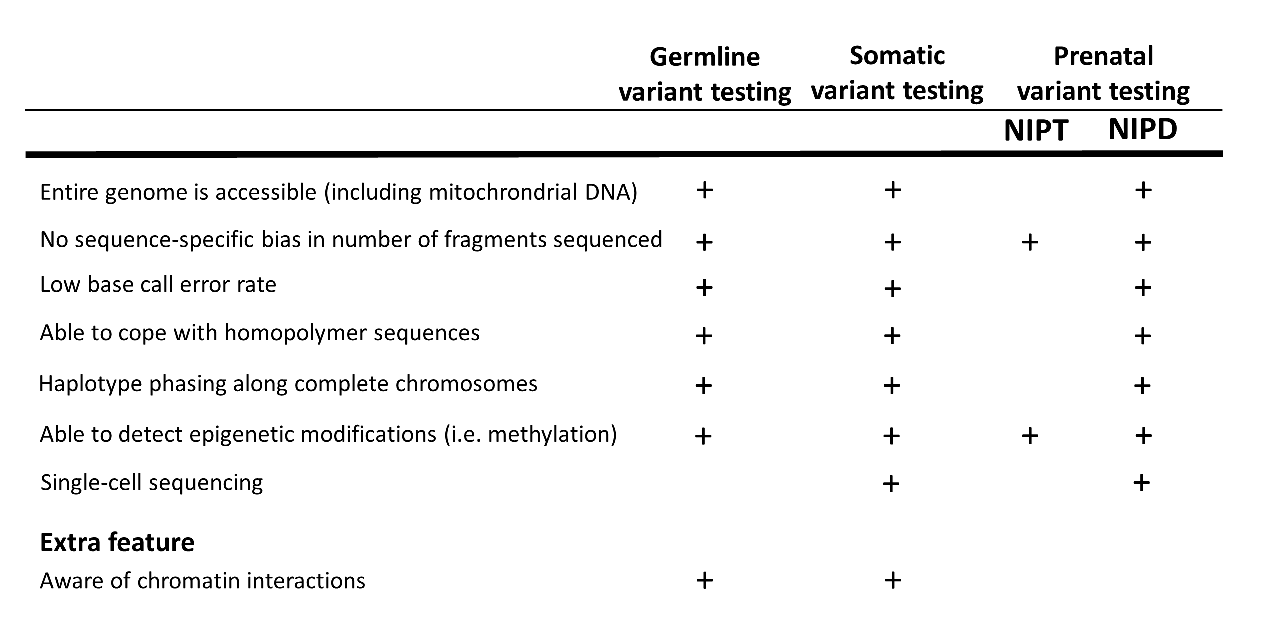
\includegraphics[width=1.0\linewidth]{img/Chapter11_table1}
	\label{table:Chapter11_table1}
\end{table}

Many of the requirements of sequencing techniques that are necessary to detect all DNA variants are similar for germline, somatic and for prenatal variant testing, but some differ (Table
\ref{table:Chapter11_table1}). 
In general, testing for germline variants is less demanding than testing for somatic variants because a lower sensitivity can suffice. 
However, it is often the case in practice that, when the main interest is in germline variants, there is also an interest in detecting somatic (mosaic) variants. 
For prenatal testing, discussion is now on-going about whether to test for variants other than the
common trisomies \cite{Bowman_Smart_2019}. In NIPT, screening is performed on cell-free DNA (cfDNA) for (sub)chromosomal abnormalities. 
However, there is also a desire for non-invasive detection of other types of DNA variants that are related to congenital conditions \cite{Hayward_2018}. 
In this discussion I use the term NIPD to describe these kind of tests. 
Because fetal cells or DNA only comprise a small part of the total cell population or DNA quantity, there is a need to identify the relevant cells or to have a high sensitivity to detect variants if mixed maternal/fetal DNA is analyzed. 
For this reason, NIPD variant calling would have identical demands to somatic variant testing.

In the following part of the discussion I first focus on the demands of germline and somatic variation detection and how both goals meet. 
I then turn my focus to prenatal variant detection and why the demands on NIPD are higher than those on NIPT. 
Many of the techniques used are still costly to perform and therefore not yet feasible for routine use. 
Here I focus primarily on the technical side of the methods and techniques and leave out discussions of the feasibility of using these techniques in daily practice.


\subsection[Short-read-sequencing-based variant detection]{Short-read-sequencing-based germline and somatic variant detection}
All of the demands that hold for complete germline variant detection are equally (or more) important in somatic variant detection. 
Massively parallel high-throughput sequencing is, in my opinion, a necessary condition to sequence the vast amount of DNA needed to detect all variants with sufficient speed. 
Sequencing costs have decreased rapidly in the past decade \cite{Wetterstrand_2018}. 
If this steep decline continues, WGS procedures may become more cost-efficient than targeted enrichment procedure. 
The availability and costs of data processing and storage would then be the main factor driving the feasibility of implementation of (routine) WGS. 

Sequencing the entire genome has several benefits compared to targeted approaches. 
First of all, obviously, more variants are called – i.e. all variants in a complete DNA sequencing procedure – making it possible to reinterpret variants when new information is available. 
For example, \textsl{CDH2} has now been associated to Arrythmogenic Right Ventricular Cardiomyopathy \cite{Mayosi_2017}.
However, because this gene was not yet associated to the disease at the time we developed our cardiomyopathy gene panel, it was not included in the gene panel in chapters 2 and 3. 
If WGS had been done for these samples, variants in this gene could have been analyzed retrospectively, possibly increasing diagnostic yield. 
A further benefit of WGS, and WES, compared to gene-panel-approaches is that all samples can be processed the same way (except filtering), thus facilitating the use of a standard workflow. 
In addition, WGS requires fewer steps in sample processing. This means less variation will be present between samples, making them easier to compare, and provides more even coverage between samples, making a larger part of the genome accessible \cite{Meienberg_2016}.
Furthermore, when performing WGS, no assumptions are made regarding the presence of certain genomic sequences. 
In targeted sequencing, only the targeted regions and regions that are close by are captured. 
Hence, targeted procedures only analyze what is expected to be present. WGS allows for a more unbiased approach. 
These gains can be achieved using the types of short-read sequencing used in this thesis. 
In addition, (short-read) WGS allows for more types of algorithms to be used. 
This is especially useful within SV calling, where, in addition to read-depth, the effect of a structural variation on reads themselves can also be analyzed, because it is more likely that a read will span (one of) the breakpoints involved \cite{Rausch_2012}. 
However, even in WGS, the length of the short-read sequence leads to the inability to sequence part of the genome \cite{Mandelker_2016}.
Given that over 50\% of the genome is made up of repeat-sequences, especially in the non-coding part \cite{Jain_2018a}, for many variants it is difficult – if not impossible – to attribute them to a specific place in the genome without further follow-up testing.

A further limitation of standard short-read sequencing is that it uses bulk-isolated DNA as input. 
In other words, the DNA of many cells is extracted and isolated as a mix. 
This makes it impossible to distinguish DNA-fragments (reads) from different cells. 
For germline variations, in general, two copies of each allele are present (i.e. two haplotypes). 
A variant is expected to be present on one or both haplotypes. For somatic variations, the situation is different. 
If, for instance, a variation is present in only 10\% of the cells, a third haplotype is present in low frequency. 
For a single variant this would only create an issue of sensitivity. 
In absence of sequencing errors, a variant present in 10\% of the cells would, for the variant location, result in 5\% of the reads containing the variant (on average). 
Given sufficient coverage, these variants can be detected in the bulk sequencing data, with the sensitivity depending on the base-call error rate. 
Several methods are available to increase sensitivity \cite{Hiatt_2013,Stahlberg_2017} and various tools are available to detect such variants in short-read sequencing data \cite{Wilm_2012,Huang_2017,Said_Mohammed_2018}, although many tools rely on comparison of DNA isolated from a tumor with matched germline DNA. 

\subsection{Single cell DNA sequencing}
If different somatic variants are present and do not fall within the same sequencing read, it may not be possible to phase the variants. 
Two un-phased variants can originate from the same cell, but also from two different cells. 
This extra layer of information can be obtained via single-cell DNA sequencing (sc-seq) using short-read NGS \cite{van_den_Bos_2018, Price_2018}. 
Currently two protocols are in place for SNV and indel detection and for CNV detection, respectively. 
Ideally though, both types of variations should be detectable using the same protocol.

Cytogenetic techniques, such as karyotyping and Fluorescence In Situ Hybridisation (FISH), are often used in the search for somatic variants because aberrations can be attributed to specific cells. 
This is especially important in the search for complex karyotypes (with multiple aberrations present in the same cell), as is often the case in hematological malignancies or solid tumors with different subclones. 
In contrast to standard (short-read) sequencing, with sc-seq all the variants detected can be assigned to a specific cell, allowing detection of complex genomic patterns. 
This would make NGS suitable for use in such situations, and it would have an advantage over cytogenetic techniques as variants can be detected up to the single-nucleotide level.

A further use of sc-seq can be in NIPD, as discussed in section 11.5.5

\subsection{Long-read sequencing}
Long-read sequencing can overcome several limitations encountered in short-read sequencing.
Similar to NGS, long-read sequencing is a catch-all phrase for sequencing techniques that enable the creation of sequence reads above the sizes provided by the short-read NGS methods. 
Apart from nested PCR using an initial long-range PCR combined with Sanger sequencing \cite{Michalatos_Beloin_1996,Tan_2012}, these are all NGS techniques. 
Existing long-read sequencing techniques such as PacBio SMRT sequencing \cite{Chaisson_2014} and Oxford NanoPore Technologies (ONT) \cite{Jain_2018a,Nanopore_2018} can already achieve read lengths up to 100 kb and over 2 Mb, respectively. 
With the costs of long-read sequencing decreasing \cite{van_Dijk_2018}, it might eventually be feasible to use these techniques for sequencing in diagnostics.

The first advantage of long-read NGS is that, for a larger part of the genome, reads can be mapped uniquely. 
This makes it possible to distinguish genes and pseudogenes and to perform haplotype phasing for long stretches of DNA (i.e. stretches of DNA, including variants, can be attributed to the same chromosome), as well as to distinguish compound heterozygous variations from variations that are present on the same chromosome. 
Furthermore, long reads permit investigation of genomic areas that have long non-unique sequences and extend the known reference sequence \cite{Ameur_2018}. 
Recently, the Y-chromosome centromere sequence was determined using ONT, despite the presence of a 5.8 kb tandem repeat of over 300 kb length in total \cite{Jain_2018b}.

A second advantage of long-read NGS is SV-detection. Because long reads (or haplotype blocks) are more likely to span breakpoints, SVs are more likely to be detected. Analysis of SVs in long reads is not straightforward, however, since multiple breakpoints are present in a single read in some cases \cite{Gong_2018,Pollard_2018}.

Current long-read NGS techniques still have limitations compared to short-read sequencing techniques. 
Short-read methods have a lower base error rate than long-read ones \cite{Chaisson_2014,Jain_2018b,van_Dijk_2018}. 
Moreover, detection of homopolymer length has a much higher error rate, even though these are problematic regions for short-read sequencing as well \cite{Laehnemann_2015, Rang_2018}. 
For now, short-read techniques are superior for detection of SNVs and indels in the accessible parts of the genome, but the best of both worlds can be achieved by using short-read sequencing to ‘polish’ the sequences inferred by long-read sequencing \cite{Jain_2018a}. 
Because the different techniques are affected by different biases, combined variant calling confidence can be higher when both techniques produce concordant results. 
Using this strategy, the Genome In A Bottle (GIAB) consortium have created reference genomes containing high-confidence calls that can be used for benchmarking tests \cite{Zook_2014,Zook_2018}. 

A key challenge at the basis of long-read sequencing is the isolation of long DNA fragments.
Currently several companies, most notably Circulomics \cite{Liu_2018}, Sage Science \cite{Shin_2018} and Revolugen \cite{Birkenhead_2018} are all developing different technologies for this purpose.

As an alternative to long-read NGS, there are techniques available to bridge the gap between short- and long-read sequencing. 
By adding molecular barcodes to short reads originating from the same DNA fragment, synthetic long reads can be created. 
One such technique is 10xGenomics genome sequencing \cite{10xGenomics_nd}. 
With synthetic long reads, the information regarding the surrounding sequence is not inferred from the same read, but from other reads having the same identifier. 
This is an important limitation, since identical sequences are located close to each other in some genomic regions, which means that some of the original fragments will contain both regions and some short reads with the same identifier will have identical sequences. 
Such reads still can’t be uniquely aligned or assembled. 
Moreover, the longer the length of the DNA fragments, the more frequently non-unique sequences will appear on the same fragment. However, synthetic long-read sequencing benefits from the low error rate of short-read sequencing and can enlarge the part of the human genome that can be accessed through short-read sequencing and add haplotype information to short-read sequencing data. 
As such, it can be interpreted as an intermediate between short- and long-read NGS.

The strength of long-read sequencing can be increased by combining different platforms. 
The most notable benefit is the length of haplotype blocks. 
If there is no overlap or difference in variants between sequencing reads for a specific genomic sequence, we cannot determine whether the two blocks on either side of that sequence belong to the same haplotype. Therefore, no phasing is possible for variants between blocks. Often, the regions in which phasing is not possible differ between techniques, thus allowing connection of haplotype blocks by combining information from
different techniques. 
A technique that has become a key player in these kinds of analyses is BioNano Next-generation Mapping \cite{Bionanogenomics_2018}. 
BioNano can analyze extremely long DNA fragments over 1 Mb of length, but it is not a sequencing technique. 
BioNano instead uses endonucleases or direct labelling to create a pattern of fluorescent labels along the DNA fragment to form so-called “molecules”. By aligning these molecules to each other, large haplotype blocks can be assembled. 
This technique has been combined with Illumina 10xGenomics synthetic long read \cite{Mostovoy_2016, Levy_Sakin_2019}, as well as with Pacific Biosystems \cite{Pendleton_2015} and ONT Nanopore \cite{Ma_2018} long read, to phase reads and create haplotype blocks as long as entire chromosome arms. 
For the same purpose, Illumina short reads prepared using TLA were combined with PacBio long reads \cite{Lawrence_2016}.

On the road to a complete DNA sequencing technology, ONT has an extra feature: it allows for detection of epigenetic alterations of nucleotides during sequencing \cite{Jain_2018a}. 
For instance, a 5-methylcytosine and a cytosine passing through a nanopore result in a different change in current allowing them to be distinguished. Putting this technology to use, researchers have already
been able to create a personal map of the complete Y-chromosome, including the CpG methylation status, by following flow cytometry with ONT combined with Illumina short-read sequencing \cite{Kuderna_2019}. 
The detection of methylation patterns can be of benefit in various ways. 
For instance, Prader-Willi syndrome and Angelman syndrome result in completely different phenotypes, but both are caused by genes in the same chromosomal region \cite{Adams_2008}. 
Patients with a deletion of this region have one of these two syndromes depending on the loss of the maternal (Angelman syndrome) or paternal copy (Prader-Willi syndrome). 
The reason for this is that the \textsl{UBE3A} gene involved in the Angelman syndrome is methylated on the paternal chromosome, and therefore not expressed. In contrast, loss of the paternal copy of the 15q11-q12 region results in Prader-Willi syndrome because the genes involved are methylated on the maternal chromosome.
Both syndromes can also be caused by a uniparental disomy or by an imprinting defect, resulting in the genes being methylated on both chromosomal copies \cite{Adams_2008}. 
Other applications of DNA methylation detection are cancer genetics and metabolic and neurological disorders \cite{Jin_2018}. 
There is also evidence that the detection of methylation patters can be used for identification of fetal alcohol spectrum disorder, possibly further extending the utility of methylation analysis \cite{Portales_Casamar_2016,Lussier_2018}. 

\subsection{Chromatin organization}
A further kind of information regarding genetic variants and their effects is to not only know which variant is present at which position in the genome, but also how they are organized in a cell. 
It is known that some parts of the genome, often located on different chromosomes, interact with each other in so-called topologically associated domains (TADs) and can be involved in gene regulation.
These TADs can be disrupted or created by a genetic variants \cite{Franke_2016,Krumm_2018}. 
Some of the points of chromatin contact are tissue-specific, corresponding to active enhancers \cite{Krumm_2018}. Information on chromatin structure may therefore aid the interpretation
of variants and connect them to disease phenotypes.

Currently, several techniques (such as 3C, 4C and HiC) are available to analyze these kinds of interactions \cite{Spielmann_2018}. 
These methods all rely on cross-linking, digesting and ligating DNA fragments, leading to a shuffled genome, but they differ in the number of associations they show \cite{de_Wit_2012}. Based on such experiments, a three-dimensional model of the human genome has been created for different cell types showing the different genomic interactions \cite{Wang_2018}. 
To assess the effect of a specific genomic variant on genomic interactions, this kind of model can aid in prioritizing variants for further analysis. 
However, to confirm such an effect for a specific variant, new experiments have to be performed.

\subsection{Prenatal variant detection}
In my opinion, for optimal non-invasive prenatal trisomy testing, sequence reads have to follow three criteria: they have to be uniquely attributable to a chromosome location, distinguishable between
fetus and mother and have as little bias in numbers as possible. 
For NIPT using cfDNA, an amplification-free analysis helps reduce laboratory-induced bias \cite{van_den_Oever_2012,van_den_Oever_2013}. 
But for cfDNA, there is no need to use long-read sequencing because only short fragments are present. 
Currently, next to low-coverage WGS based analysis, targeted strategies are used that utilize SNP information to estimate the percentage of fetal DNA \cite{Stokowski_2015,Brady_2015}. 
As discussed in chapter 8, knowing the percentage of cell-free fetal DNA (cffDNA) helps to more accurately determine the personalized posterior risk of the test. 
Moreover, by determining which cases have a low percentage of cffDNA (e.g. \textless4\%), cases in danger of producing a false negative result can be identified. 
Different tools have been created to perform such estimations in low-coverage WGS NIPT \cite{Peng_2017}, some of them using biological differences between the DNA of the mother and placental DNA to differentiate between maternal cfDNA and cffDNA. Due to different sites of DNA breakage in the linker region between nucleosomes, placental DNA is, on average, shorter than maternal DNA. 
Therefore, any fetal chromosomal aberration should be present in a higher percentage of short fragments compared to longer fragments \cite{Yu_2014b,Yu_2016}. 
Furthermore, the sites at which the placental DNA breaks are not random due to the higher accessibility of nucleosome cores in the placenta \cite{Sun_2018a}. 
This means that reads located on certain genomic locations have a very high probability of being of placental origin. 
Using this information, the fraction of cffDNA can be estimated \cite{Straver_2016}, although this strategy is less reliable than using the Y-chromosomal fraction in pregnancies with a male fetus \cite{van_Beek_2017}. 
Furthermore, the preferred end-sites can be used to discriminate fetal aberrations from maternal aberrations \cite{Sun_2018a}. 
Alternatively, differential methylation between maternal and placental DNA can be used to estimate fetal fraction \cite{Nygren_2010}.

While these methods hold great promise for prenatal detection of aneuploidies and CNVs using a non-invasive procedure, as is the case in NIPT, they are unsuitable for NIPD, where SNVs and indels need to be detected in a large number of genes. Recently, using a targeted capturing panel for 30 genes associated with frequent Mendelian dominant disorders, de novo and paternally inherited variants were detected with high sensitivity and specificity in a small set of samples \cite{Zhang_2019}. 
However, the utility of this strategy may be limited for regions in which there is a relative under-representation of fetal DNA compared to maternal DNA because of the preferred end-sites.
Moreover, the sensitivity to detect maternally inherited variants will be very low because these variants have to be detected against a high background of variants in maternal cfDNA. 
To overcome this issue, haplotype information of the mother’s genome can be used to enable phased variants to serve as a proxy for a variant of interest \cite{Vermeulen_2017,Jang_2018}. 
These methods are used for monogenic disorders for which it is known that the mother is a carrier. 
Currently it is still too expensive to perform such experiments on a whole-genome- or whole-exome-basis in a diagnostic setting. 
Alternatively, NIPD could be performed on trophoblast cells from a Papanicolaou (PAP) smear \cite{Jain_2016}. 
It is possible that these cells could provide a source of high molecular DNA suitable for long-read sequencing and single-cell sequencing. 
In addition, these cells may provide a basis for analysis of the trophoblast DNA methylation status. 
The detection of methylation of embryonic single-cells is already possible \cite{Zhu_2017}. 
This extra layer of information may provide information on imprinting disorders and early-life neurodevelopmental programming, which are predictive for the development of cognitive impairments \cite{Kotzot_2007,Tilley_2018}. 
Such a broad diagnostics analysis may be too comprehensive to use for population screening. 
In addition, because of confined placental mosaicism, it is not clear what the predictive value of the test would be. 
Therefore, we should consider limiting its availability to only those pregnancies in which there is a prior indication of the presence of a pathogenic variant, such as the presence of ultrasound abnormalities or a family history of a specific hereditary condition. 

\section{Point-of-care testing}
A different development that may continue in the future is point-of-care analysis \cite{Roberts_2012}. 
In other words, rapid genetic analysis for specific genes or variants that can be performed at the bedside. 
Here, the focus is on specific variants that are expected, so that a targeted test can be performed. 
For NGS, very small sequencers are already available, such as the ONT MinION and the SmidgION, that can be used in the most barren conditions \cite{Johnson_2017}. 
In addition, many different methods have been developed to enable such detection, but robustness, sensitivity and specificity is still limited and processing is not yet fast enough \cite{Zhang_2018}. 
I expect that in the future, these limitations will be overcome and these methods will be used to answer specific questions in human genetics, such as detection of relevant variants in pharmacogenetics, and personalized cancer medicine \cite{Dancey_2012}. 
A different application may be confirmation of carriership of specific variants. 
If it is known that a specific genetic variant is common in a geographic region with limited access to genetic testing, then point-of-care testing for that variant may provide the possibility to diagnose people who would otherwise not have the opportunity for treatment. 

\section{Looking towards the future}
It seems that, when putting all the current technologies in the mix, we already come close to meeting the demands I posed upon a complete DNA sequencing technology, at least regarding germline
variation detection. 
At the moment, however, many different experiments need to be performed, each answering just part of the puzzle. 
This means that it is expensive and time-consuming to get the total package of information. 
I believe it is feasible to create a single test to perform a single-cell analysis of the DNA sequence of complete chromosomes and mitochondrial DNA, with a low base call error rate and the capacity to detect base modifications. 
Considering that it is already possible to select single cells, it is easy to imagine a nanopore-based technique where, for instance, cells are first captured in a grid of wells, each able to contain a single cell. 
Cells could then be lysed and DNA freed into the well without (too much) breakage. 
If those wells would contain nanopores, the intact DNA, including base modifications, could be measured. 
If each DNA strand is measured multiple times, the base call error rate can be massively reduced and, because each cell in principle only contains two copies of each chromosomes, phasing should be easy. 
If tumor cells are sequenced in this way, the higher complexity of karyotypes would make analysis more difficult, especially if two identical chromosomes are present through replication. But, if each chromosome (or mitochondrial genome) in the cell is sequenced often enough, it can be expected that in cases of aneuploidies certain chromosomes would be sequenced more often than others. 
Such a test would fulfill almost all the properties of a complete DNA sequencing technique, although homopolymers may still pose a challenge and the three dimensional structure will not be measured by this technique.

In the past few years the value of multi-omics approaches that can provide information on the relations between genetic variants and variability in the epigenome, transcriptome, proteome, metabolome or microbiome has been shown \cite{Hasin_2017}. 
If we take our wish list one step further and take our focus off of DNA analysis, the open chromatin, transcriptome, metabolome and proteome of the cell could be measured in the same experiment. 

Going to an amplification-free single-cell DNA analysis technique with ultra-long reads will drastically reduce laboratory and sequencing noise and thereby data analysis noise. 
However, it has no influence on biological noise and, for optimal results, the demands on the input material are high.
If the input material contains fragmented DNA (e.g. FFPE material) the technique performs suboptimally, possibly leading to incomplete phasing of chromosomes. 
In addition, variants that occur in the DNA through transversion (i.e. C $\leftrightarrow$ A or G $\leftrightarrow$ T change) that has occurred during long-term storage will be detected as real variants. On the other hand, a complete DNA sequencing technique would get the most out of the available input material.
I believe that point-of-care genetic testing will further develop for testing of specific (sets of) variants, such as in pharmacogenetics. 
Mobile sequencers are already in existence and can be used almost anywhere on the planet. 
These developments will help introduce genetic testing in currently underrepresented areas.

\section{Conclusion}
In this thesis we have pursued several strategies to improve genetic variant detection in various sources of material. 
We set up and implemented laboratory procedures and introduced novel algorithms. 
We have demonstrated that these methods and tools can reliably detect different types of variants. 
Partly, the methods and algorithms introduced in this thesis are suitable to replace, or have already replaced, conventional methods as a first-line method. 
For instance, our targeted NGS gene panels replaced Sanger sequencing and MLPA as first-line methods and NIPT has been implemented as an alternative to amniocentesis and chorionic villi biopsy analysis. 
The TLA multiplex panel has shown promising results for detection of somatic chromosomal translocations, but has not surpassed conventional methods in sensitivity and specificity for detection of those variants. 
In the final part of the thesis, I have reflected on the epistemological status of knowledge generated through NGS and investigated which moral implications the introduction of the methods introduced in this thesis may have. 
Finally, I have pondered the status of short-read sequencing in the future.
Because of the greater accessibility of the genome using longer reads, these techniques might take over in the future, given sufficient quality and cost-effectiveness. 
Furthermore, sequence information and epigenetic nucleotide alterations can already be inferred during a single experiment. 
Techniques enabling such experiments may turn out to be the future of genome sequencing because they allow us to answer multiple questions at the same time, a characteristic that may be invaluable to cope with the complexity of genomic diseases.